Today's data are shown in Fig. \ref{fig:today}, and yesterday's data are
shown in Fig. \ref{fig:yesterday}.

\begin{figure}[htbp]
\centering
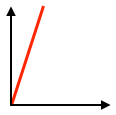
\includegraphics{img/today.png}
\caption{Today's \(y=mx+b\) data.\label{fig:today}}
\end{figure}

\begin{figure}[htbp]
\centering
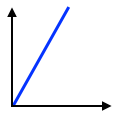
\includegraphics{img/yesterday.png}
\caption{Yesterday's \(y=mx+b\) data.\label{fig:yesterday}}
\end{figure}

Earlier data are shown in Fig. \ref{fig:earlier}. Fig.
\ref{fig:earlier}a is for two days ago and Fig. \ref{fig:earlier}b is
for three days ago.

\begin{figure}[htbp]
\centering
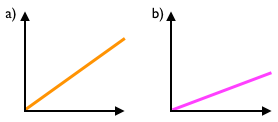
\includegraphics{img/earlier.png}
\caption{Data from a) two days ago, and b) three days
ago.\label{fig:earlier}}
\end{figure}

Figures \ref{fig:today}--\ref{fig:earlier}
(\ref{fig:today},\ref{fig:yesterday},\ref{fig:earlier}) reveal an
increasing slope with time.
